\section{Product perspective}
\label{sec:product_perspective}%

\subsection{Class Diagrams}
\label{subsec:class_diagrams}%
The diagram below represents and describes the classes involved in the system, their basic functionalities, attributes,
and the relationships between them.
From the diagram, it is easy to see how the tournament entity function as a bridge between different
components. More specifically, in our design we assigned to this entity the task to hold track 
of battles, leaderboard of the tournament itself and badge assignment.
All the other functionalities are esily understandable from within the diagram or 
will be later discussed. \newline
Here, we want to stress that, even though just an high level view of the system-to-be, some consideration of implementation can be done. 
More specifically, some design pattern can be taken into consideration:
\begin{itemize}
    \item Decorator Pattern: to implement the logic behind the scoring system. Educator's choice of different aspect to consider will be easily managable 
    \item Observer patter: to implement the structure behind the notification system.
    \item Factory pattern: for the creation of different Badges with different characteristics and requirements.
  \end{itemize}

\begin{figure}[H]
    \begin{center}
        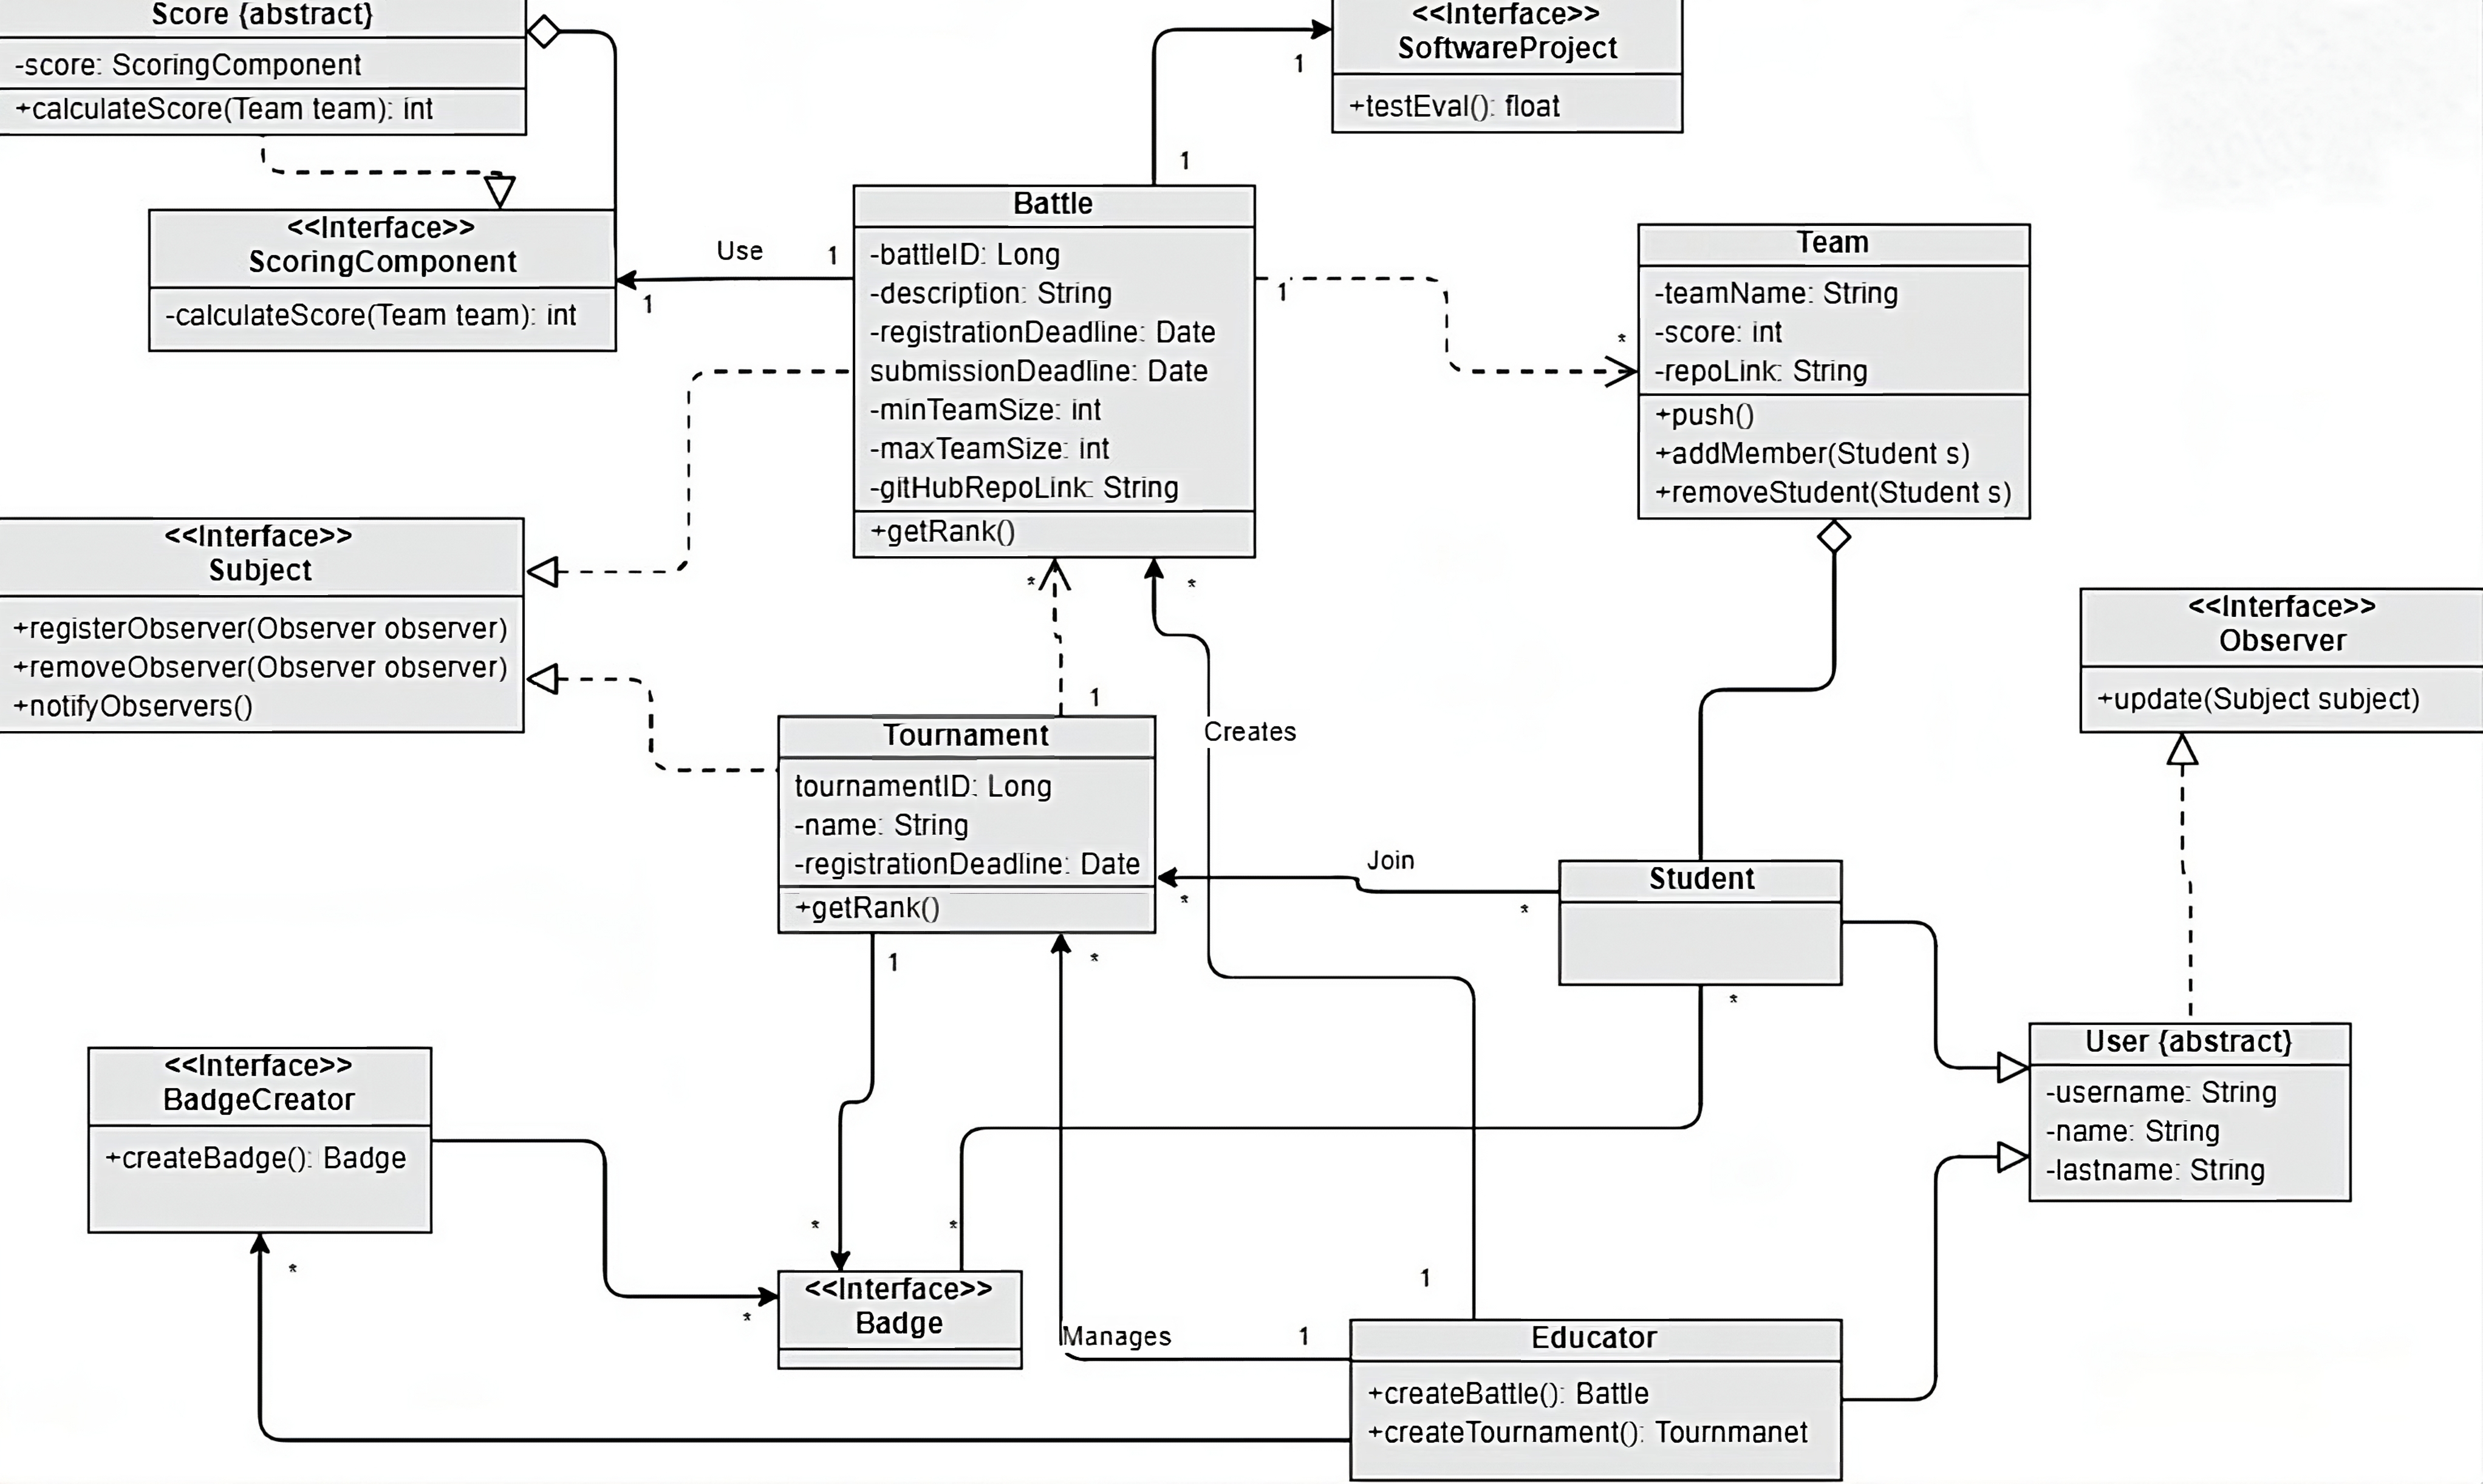
\includegraphics[width=0.9\linewidth]{Images/class-diagram.jpeg}
        \caption{A simplified Class Diagram}
        \label{fig:class_diagram}%
    \end{center}
\end{figure}

\subsection{State Diagrams}
\label{subsec:state_diagrams}%


\subsection{Scenarios}
\label{subsec:scenarios}%

\paragraph{Unregistered student creates an account.}
Gianmarco is a computer science student from Politecnico of Milan. After attending several courses about software engineering, 
he is looking for a way to practice his skills. Fortunately, one of his professor suggests him the CodeKataBattle platform.
Gianmarco immediately proceeds to create an account. He navigates to the platform and goes to the "sign up" section. 
The system asks Gianmarco some personal information such as first and last name, an email linked 
to an institutional profile (for example name.surname@mail.polimi.it). He receives an e-mail with a 
6-digit code to be in inserted in the web page to confirm his e-mail address. In the meanwhile, the platform 
receives information about the status of Gianmarco from the university (wether he is a teacher or a student). 
After accepting the terms \& conditions 
and submitting an username for his profile, the system creates his account, and Gianmarco can begin to use the platform.

\paragraph*{User Logs in.}
Emily, the coding enthusiast, is all set for her daily dose of challenges on the CodeKataBattle (CKB) platform. 
To embark on her coding adventure, she clicks the login button and enters her institutional email.
The platform asks Emily to provide the password for her account. 
Excited and confident, Emily types in her password, which is verified by the platform to ensure it matches the email/password combination for the user.
With a successful password match, the platform welcomes Emily to her homepage; she's now ready to dive into the coding battles.
In case there's a typo in her email or a hiccup during password verification, the platform gently guides Emily through the process, ensuring a seamless login experience.

%Actor Student
%Entry conditions The student is logged in on the CKB platform.
%Event Flow 1. The student clicks on the "Create team" button from the tour-
%nament page.
%2. The CKB platform prompts the student to input the size of the
%team.
%3. The student inputs the size of the team.
%4. The CKB platform prompts the student to input the name of the
%team.
%5. The student inputs the name of the team.
%6. The CKB platform checks the name of the team.
%7. The CKB platform communicates the outcome of the team cre-
%ation.
%Exit condition A team is created.
\paragraph*{Student creates a team.}
Francesca, a student on the CodeKataBattle (CKB) platform, is eager to participate in the "Algorithmic Challenge" CKB.
Francesca is aware that winning the battle all by herself is a daunting task, so she decides to form a team.
She navigates to the tournament details page and clicks on the "Create Team" button and is prompted to input the size of the team.
Francesca wants to form a team of three students, so she chooses the number three from the drop-down menu.
After deciding that the name of her team will be "The Three Musketeers," she clicks on the "Create Team" button.
She will now need to choose to whom she wants to send the team invitation.


%Actor Student
%Entry conditions The student is logged in on the CKB platform and created a team.
%Event Flow 1. The student selects a student from the list of students on the
%tournament page.
%2. The student clicks on the invite button on the bottom of the list
%of students from the tournament page.
%3. The CKB platform checks for remaining space in the team.
%4. The CKB platform sends the invitation to the selected student.
%5. The CKB platform communicates the outcome of the invitation
%to the student.
%Exit condition An invitation is sent.
\paragraph*{Student invites another student to join a team.}
Imagine Marco, an enthusiastic student navigating the CodeKataBattle (CKB) platform, keen on forming a proficient coding team for an upcoming tournament. 
Having already gathered part of his team, Marco identifies Sofia, another student he believes would enhance their collective skills.
On the tournament page, Marco locates Sofia's profile and clicks the "Invite" button, signaling his desire to collaborate. 
The CKB platform efficiently checks team capacity, ensuring seamless integration.
In the digital realm, an invitation is generated and dispatched to Sofia through the platform's communication channels. 
Marco eagerly awaits the platform's response, hopeful for a positive outcome.
Success! The invitation is sent, propelling Marco's team towards a cohesive coding alliance.



\paragraph*{Student accepts an invitation to join a team.}
Sofia, a student passionate about coding, is actively using the CKB platform to participate in coding tournaments. 
Today, as she's logged in, he receives a pop-up notification indicating that she has been invited by Marco to join a team for a CKB.
Intrigued, she clicks on the "Accept" button within the invitation pop-up as she knows that her and Marco would be a good team. 
Behind the scenes, the CKB platform swiftly processes this action and conveys the acceptance information to the student who sent the invitation, ensuring a seamless interaction between both students involved.
Alex and the sender of the invitation are promptly notified of the outcome. 
The invitation has been successfully accepted, and Sofia is now part of the team.



\paragraph*{Student rejects an invitation to join a team.}
Sofia, a dedicated student engaged in coding challenges on the CKB platform, is logged in and actively participating. 
Today, she receives a pop-up notification, signaling that she has received an invitation to join a coding tournament.
After thoughtful consideration, Sofia decides to decline the invitation. 
With a click on the "Reject" button within the invitation pop-up, she communicates her decision to the CKB platform. 
Behind the scenes, the platform ensures this information is promptly relayed to the student who extended the invitation.
Both Sofia and the sender of the invitation receive immediate communication from the CKB platform, confirming the outcome of the declined invitation. 
The respectful rejection is acknowledged, allowing the students to proceed with their individual coding journeys.


\paragraph*{Student joins a battle without a team.}
Emma, an enthusiastic student with a passion for coding challenges, is actively participating in a coding tournament on the CKB platform. 
Excited about a specific battle, she navigates to the tournament page to explore the available challenges.
Spotting a captivating battle in the list, Emma decides to join without forming a team as she is confident on her own skills. 
She selects the desired battle and clicks the "Join Battle" button at the bottom of the list.
Behind the scenes, the CKB platform promptly verifies the registration deadline for the chosen battle. 
Upon completion of this process, the platform communicates the outcome of Emma's action. 
Whether met with success or needing adjustment, Emma receives immediate feedback, allowing her to seamlessly engage in the selected coding challenge.


\paragraph{Professor creates a tournament. }
Achille is a cyber security professor from university of Milan. He has an active profile on the CKB platform. 
During his last lesson, he annouced to his students that he will create monthly tournaments with weekly Battle for them to practise. 
He then proceeds to create the first tournament. He logs in the CKB platform from the "sign-in" page. 
Then, from the menu option in the home page, he selects "Create a new tournament". He is prompted with the page of the setup for the tournament itself. 
Achille enters a name for the tournament and the registration deadline. He then toggles the "advanced options" section. 
From here, he can decide wheter to include or not badges, and, in the first case, which badges are available in the tournament. 
Achille is prompted with a set of pre-existing badges (created from the platform or in previous tournaments). He can decide to 
create new badges in addition to the ones already present. When choosing to create a new badge, a pop-up window appears where he can select and combine 
variables and rules to obtain the new badge. Once he finishes setting up everything, he pushes the "Create tournament" button at the bottom of the page. 

\paragraph*{Professor closes a tournament.}
Logged into the CKB platform, Professor Lucia navigates to the "Tournaments" page. She locates the "Programming Prodigy Challenge" in the list and clicks
on it to access the tournament details. Satisfied with the students' participation and battle outcomes, she clicks the "Close Tournament" button.
A confirmation pop-up appears, and without hesitation, Professor Lucia confirms the action. The CKB platform processes the request, communicates 
the successful tournament closure, and computes the final ranking based on accumulated scores.
The platform promptly makes the final ranking available for participants. Professor Lucia, acknowledging the students' efforts, briefly reviews the rankings. 

\paragraph*{Professor creates a new CKB.}
Professor Roberto, logged into his CKB platform account, navigates to the tournament's details page named "Algorithmic Mastery Challenge." 
Excited to introduce a new coding challenge, he clicks on the "Create New Code Kata Battle" button. 
Professor Roberto is prompted to upload a code kata for the battle: he selects a well-prepared code kata that includes a comprehensive description and a software project with test cases and build automation scripts. 
He ensures that all necessary components are included before uploading.
Then he decides that groups should consist of a minimum of two students and a maximum of four students for this battle, so Professor Roberto sets these values accordingly in the "Group Size" field.
The educator proceeds to set a registration deadline and a final submission deadline, providing students with ample time to prepare and submit their solutions.
Curious about the advanced scoring options, Professor Roberto clicks on the "Additional Configurations for Scoring" button. 
The platform displays the scoring section, allowing him to set additional configurations if needed. 
Satisfied with the default scoring, he proceeds to click the "Create" button.

\paragraph*{Professor grants permissions to another professor to add CKB to a tournament.}
Professor Marta, logged into her CKB platform account, navigates to the details page of the tournament named "Coding Challenge Extravaganza," which she initiated. 
Realizing the workload involved in creating battles, she decides to grant permissions to another educator, Professor Elena.
She clicks on the "Add Administrator" button, prompting the CKB platform to request the email or username of the educator to whom she wants to grant permissions. 
Professor Marta confidently inputs Professor Elena's email.
Professor Elena receives a notification from the CKB platform, informing her that she has been granted permissions to add battles to the tournament named "Coding Challenge Extravaganza."
Now, Professor Elena, can access the tournament details page and contribute by creating new Code Kata Battles. 

\paragraph*{Professor creates a new Badge.}
Professor Sofia, logged into her CKB platform account and currently on the details page of the "Coding Excellence Showcase" tournament, is inspired to introduce a special badge for outstanding performances. 
Excited about the idea, she clicks on the "Create New Badge" button located in the "Advanced Options" section.
The CKB platform prompts her to input the title of the badge. 
Professor Sofia, with a clear vision in mind, names the badge "Elite Coder."
Next, the platform allows Professor Sofia to define the rules for the badge. 
She navigates through a user-friendly wizard, creating rules that capture exceptional coding skills. 
Each rule represents a milestone that, when achieved, contributes to earning the "Elite Coder" badge.
Professor Sofia completes the rule-setting process, ensuring a fair and challenging criteria for students to meet. 
Satisfied with her creation, she clicks on the "Create" button.

\paragraph*{Professor manually evaluates teams in a CKB.}
Professor Marco, logged into his CKB platform account and currently on the details page of the "Algorithmic Challenge" CKB, a challenge that is ended and is in post evaluation phase.
The team already has a score, automatically computed by the platform, but Professor Marco wants to provide a more detailed evaluation. 
Eager to ensure a fair evaluation, he clicks on the "Manually Evaluate Teams" button.
The platform presents him with a list of teams that participated in the "Algorithmic Challenge." 
Professor Marco carefully selects a team from the list, keen on assessing their coding skills and approach to the given challenge.
Upon selecting a team, the CKB platform displays the team's submitted sources. 
Professor Marco thoroughly reviews the materials and, based on his expert judgment, assigns a comprehensive score to the team's performance.
Satisfied with the evaluation, Professor Marco clicks the "Save" button to record his assessment. 
This meticulous manual evaluation process repeats as Professor Marco proceeds to assess other teams involved in the "Algorithmic Challenge." 
Each score contributes to the overall ranking of the teams.

\paragraph*{User consults the leaderboard of a tournament.}
Sofia, an active user on the CodeKataBattle (CKB) platform, decides to check the current ranking of the "Data Structures Madness" tournament. 
She navigates to the "Tournaments" page and selects "Data Structure Madness" tournament.
Sofia proceeds opening the details page and effortlessly views the real-time leaderboard with a single click. 
The platform promptly presents the current standings, allowing Sofia to gauge the performance of each student subscribed to the tournament.

\paragraph*{User views the profile of another user to check their badges.}
Francesca, a student on the CodeKataBattle (CKB) platform, is intrigued to explore the profile of a student, Alex, to gain insights into his achievements. 
With a simple click on Alex's profile from the "Users" page, Francesca is presented with a comprehensive view. 
The platform seamlessly showcases the badges earned by Alex. 
To delve deeper, Francesca clicks on a specific badge and is presented with a detailed description of the badge and the criteria for earning it.

\paragraph*{User views the ranking of an ongoing CKB.}
Emma, an enthusiastic student on the CKB platform, is eager to witness the live dynamics of an ongoing coding tournament.
Logging into CKB, Emma navigates to a specific tournament, selecting a Code Kata Battle (CKB) of interest.
Within the chosen CKB, Emma clicks on "Ranking". In an instant, the CKB platform reveals the real-time rankings, showcasing the fluid movements of teams based on their pushes to the repository, automatically evaluated by the system.


\section{User characteristics}
\label{sec:user_characteristics}%
The CKB platform caters to various user roles, each with specific responsibilities and access levels:
\begin{itemize}
    \item \textbf{Guest:}  Users who are not registered on the CKB platform but have the potential to become either students or educators. 
    Guests have limited access and functionality until they complete the registration process. 
    Once registered, they can assume the roles of either Student or Educator based on their role in the institution they belong to.
    \item \textbf{Educator:} Educators who have successfully registered within the CKB system. Identified by a unique identifier, registered educators, depending on permissions granted, may assume the role of Tournament Administrator. 
    They possess the ability to create CKBs, evaluate student submissions, and engage in other system functionalities.
    \item \textbf{Student:} Users, both registered and unregistered, participating in code kata battles facilitated by the CKB platform. 
    Students can form teams, submit solutions, and engage in the competition. 
    Their scores, rankings, and achievements contribute to their overall performance, visible in the context of tournaments.
    \item \textbf{Tournament Administrator:} Educators with privileges to perform actions within a specific Tournament. Tournament Administrators, typically the creators of a Tournament, can delegate administrative powers to other educators. 
    These administrators have the authority to initiate new CKBs, evaluate submissions, and oversee tournament-related activities.
\end{itemize}

\section{Assumptions, Dependencies, and Constraints}
\label{subsec:Assumptions, Dependencies, and Constraints}%
\subsection{Assumptions}

\newcounter{ac}
\setcounter{ac}{0}
\newcommand{\ca}{\stepcounter{ac}\theac}

\newcommand{\myrow}[1]{
    A\ca & #1 \\
    \hline
}

\begin{center}
    \begin{longtable}{ |l|p{0.9\linewidth}| }
        \hline
        \textbf{ID} & \textbf{Domain Assumptions}                                                                   \\
        \hline
        D\ca        & Users, both students, and educators provide accurate personal information during the registration process.\\
        \hline
        D\ca        & GitHub repositories are assumed to support the necessary features for forking and setting up automated workflows through GitHub Actions.\\
        \hline
        A\ca        & Educators are expected to have the ability to evaluate the work done by students and assign scores if manual evaluation is required. \\
        \hline
        A\ca        & Educators managing a torunament will not lose access to their institutional email during the whole duration of the tournament itself.                                                             \\
        \hline
        A\ca        & Educators and students have a good understanding of GitHub and GitHub actions.                                  \\
        \hline
        A\ca        & Educators are capable of creating and closing tournaments, without leaving them open undefinetly.                      \\
        \hline
        \caption{Assumptions.}
        \label{tab:assumption_tab}%
    \end{longtable}
\end{center}
